\documentclass[11pt,a4paper]{report}

\usepackage[spanish]{babel}
%\usepackage[math,light]{iwona}
\usepackage[utf8]{inputenc}
\usepackage{amsmath, amsthm}
\usepackage{amsfonts, amssymb, latexsym}
\usepackage{enumerate}
\usepackage[usenames, dvipsnames]{color}
\usepackage{graphics,graphicx, float} %para incluir imágenes y colocarlas
\usepackage{colortbl}
\usepackage{graphicx}
\usepackage{wrapfig}
\usepackage[top=4cm]{geometry}
\usepackage{cite}
\usepackage[official]{eurosym}
\usepackage{cancel}
\usepackage{subfigure}
\usepackage{tikz}
\usepackage{pseudocode}
% \usepackage{multirow}

\theoremstyle{plain}
\newtheorem{exe}{Ejercicio} % reset theorem numbering for each chapter

\theoremstyle{definition}
\newtheorem{sol}{Solución}

\usepackage[bookmarks=true,
            bookmarksnumbered=false, % true means bookmarks in
                                     % left window are numbered
            bookmarksopen=false,     % true means only level 1
                                     % are displayed.
            colorlinks=true,
            linkcolor=webblue,
            citecolor=red]{hyperref}
\definecolor{webgreen}{rgb}{0, 0.5, 0} % less intense green
\definecolor{webblue}{rgb}{0, 0, 0.5}  % less intense blue
\definecolor{webred}{rgb}{0.5, 0, 0}   % less intense red

\setlength{\parindent}{0pt}
\setlength{\parskip}{1ex plus 0.5ex minus 0.2ex}

\newcommand{\HRule}{\rule{\linewidth}{0.5mm}}

\begin{document}


\begin{titlepage}

\begin{center}

% parte superior de la página
\begin{minipage}{0.4\textwidth}
\begin{flushright}
$\qquad$\htmladdnormallink{
\includegraphics[width=0.25\textwidth]{./ugr}}
      {ugr.es}\\[1cm]
\end{flushright}
\end{minipage}
\begin{minipage}{0.4\textwidth}
\begin{flushleft}
$\qquad$\htmladdnormallink{
\includegraphics[width=0.25\textwidth]{./etsiit}}
      {ugr.es}
\end{flushleft}
\end{minipage}
~\\[1cm]

\textsc{\LARGE Trabajo de Fin de Grado}\\[1.5cm]
\textsc{\Large Escuela Técnica Superior de Ingeniería Informática y Telecomunicaciones}\\[0.5cm]
\textsc{\Large Universidad de Granada}\\[0.5cm]


% título
\HRule \\[0.4cm]
{\huge\bfseries Generación Automática de los Horarios}\\[0.4cm]

\HRule \\[1.5cm]

% autor y supervisor
\begin{minipage}{0.4\textwidth}
\begin{flushleft} \large
\emph{Autor:}\\
\textsc{Braulio Vargas López}\\
\textsc{Marta Gómez Macías}
\end{flushleft}
\end{minipage}
\begin{minipage}{0.4\textwidth}
\begin{flushright} \large
\emph{Supervisor:} \\
Dr.~\textsc{Joaquín Fernández Valdivia}
\end{flushright}
\end{minipage}

\vfill

% parte inferior de la página
{\large \today}

% \vspace{5mm}

%       %\footnotesize
%       \htmladdnormallink{
\includegraphics[width=2cm]{88x31.jpg}}
%       {http://creativecommons.org/licenses/by-nc-sa/3.0/}\\
%       \texttt{Lecciones sobre Orientación by 
%       \href{mailto:mi_direccion@hotmail.com}{L. Vargas}
%       is licensed under a \htmladdnormallink{Creative Commons
%       Reconocimiento-NoComercial-CompartirIgual 3.0 Unported License}
%       {http://creativecommons.org/licenses/by-nc-sa/3.0/}
%       Permissions beyond the scope of this license may be available at
%       \htmladdnormallink{L. Vargas}{http://www.mi_web.com}}.

\end{center}

\end{titlepage}

\tableofcontents

% Descripción de sistemas "privativos"

\chapter{Descripción de otros sistemas software similares}

\section{Lantiv Scheduling Studio}

El software llamado \href{http://www.schedulingstudio.com/}{\textit{Lantiv Scheduling Studio}} es una herramienta para realizar horarios de forma \textbf{no automatizada}. Permite usar variables tales como profesorado, número de alumnos, aulas o equipamiento y, al realizar una modificación en el horario realizado, confirma que no hay ninguna incompatibilidad.

Permite realizar un calendario semanal, bisemanal o programar actividades para días concretos. Además, también permite elegir las horas a las que empieza y acaba cada actividad y, por último, también permite programar los descansos y su duración.

Respecto a su interfaz, permite cambiar el idioma y la combinación de colores que ésta usa. Al ser un programa genérico, incluye herramientas y ejemplos para hacer horarios en todo tipo de instituciones. El software puede configurarse para trabajar en un servidor (usando la IP y el puerto del mismo, además de un usuario y una contraseña), de manera que todas las personas que trabajen sobre el mismo horario puedan ver los cambios que se realizan en éste en tiempo real.

Toda esta información puede encontrarse en la documentación del software \cite{lantiv}.

\section{Mimosa}

El software llamado \href{http://www.mimosasoftware.com/}{\textit{Mimosa}} es una herramienta para realizar horarios de forma \textbf{automatizada}. A partir de información que el usuario debe introducir a mano, este software genera un horario usando algoritmos de optimización. Dicha información es: clases, profesores, salas especiales, equipo, asignaturas y alumnos. 

En la \hyperref[mimosa]{Figura \ref*{mimosa}} vemos varios pantallazos de su interfaz en la que hay varias áreas principales: una para introducir la información relativa al horario (referida en el software como \textit{recurso}), otra para añadir las asignaturas y una para ver los horarios creados. En ésta última sección podemos filtrar el horario por grupo, profesor o aula.

\begin{figure}[!h]
    \centering
    \mbox {
    \subfigure[Sección de recursos]{
    \label{recursos}
    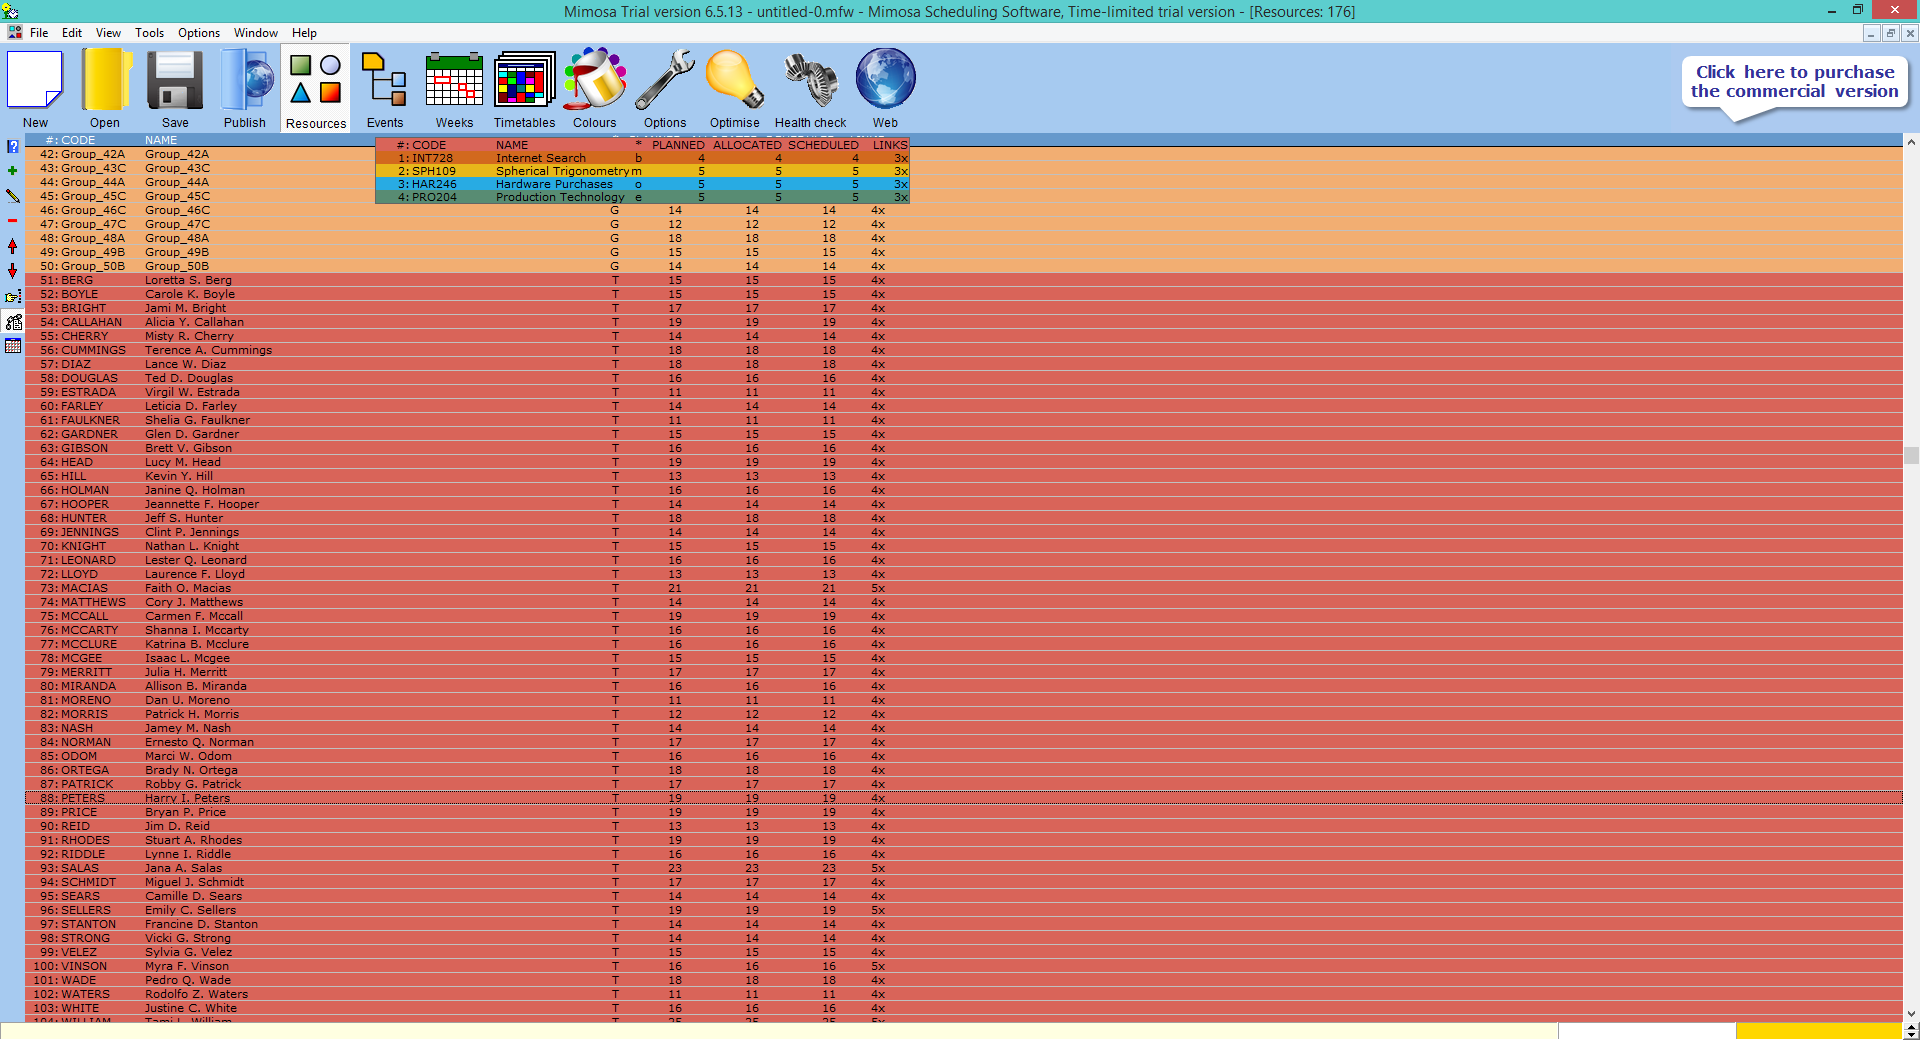
\includegraphics[width=0.5\textwidth]{1}
    }
    \qquad
    \subfigure[Sección de asignaturas]{
    \label{eventos}
    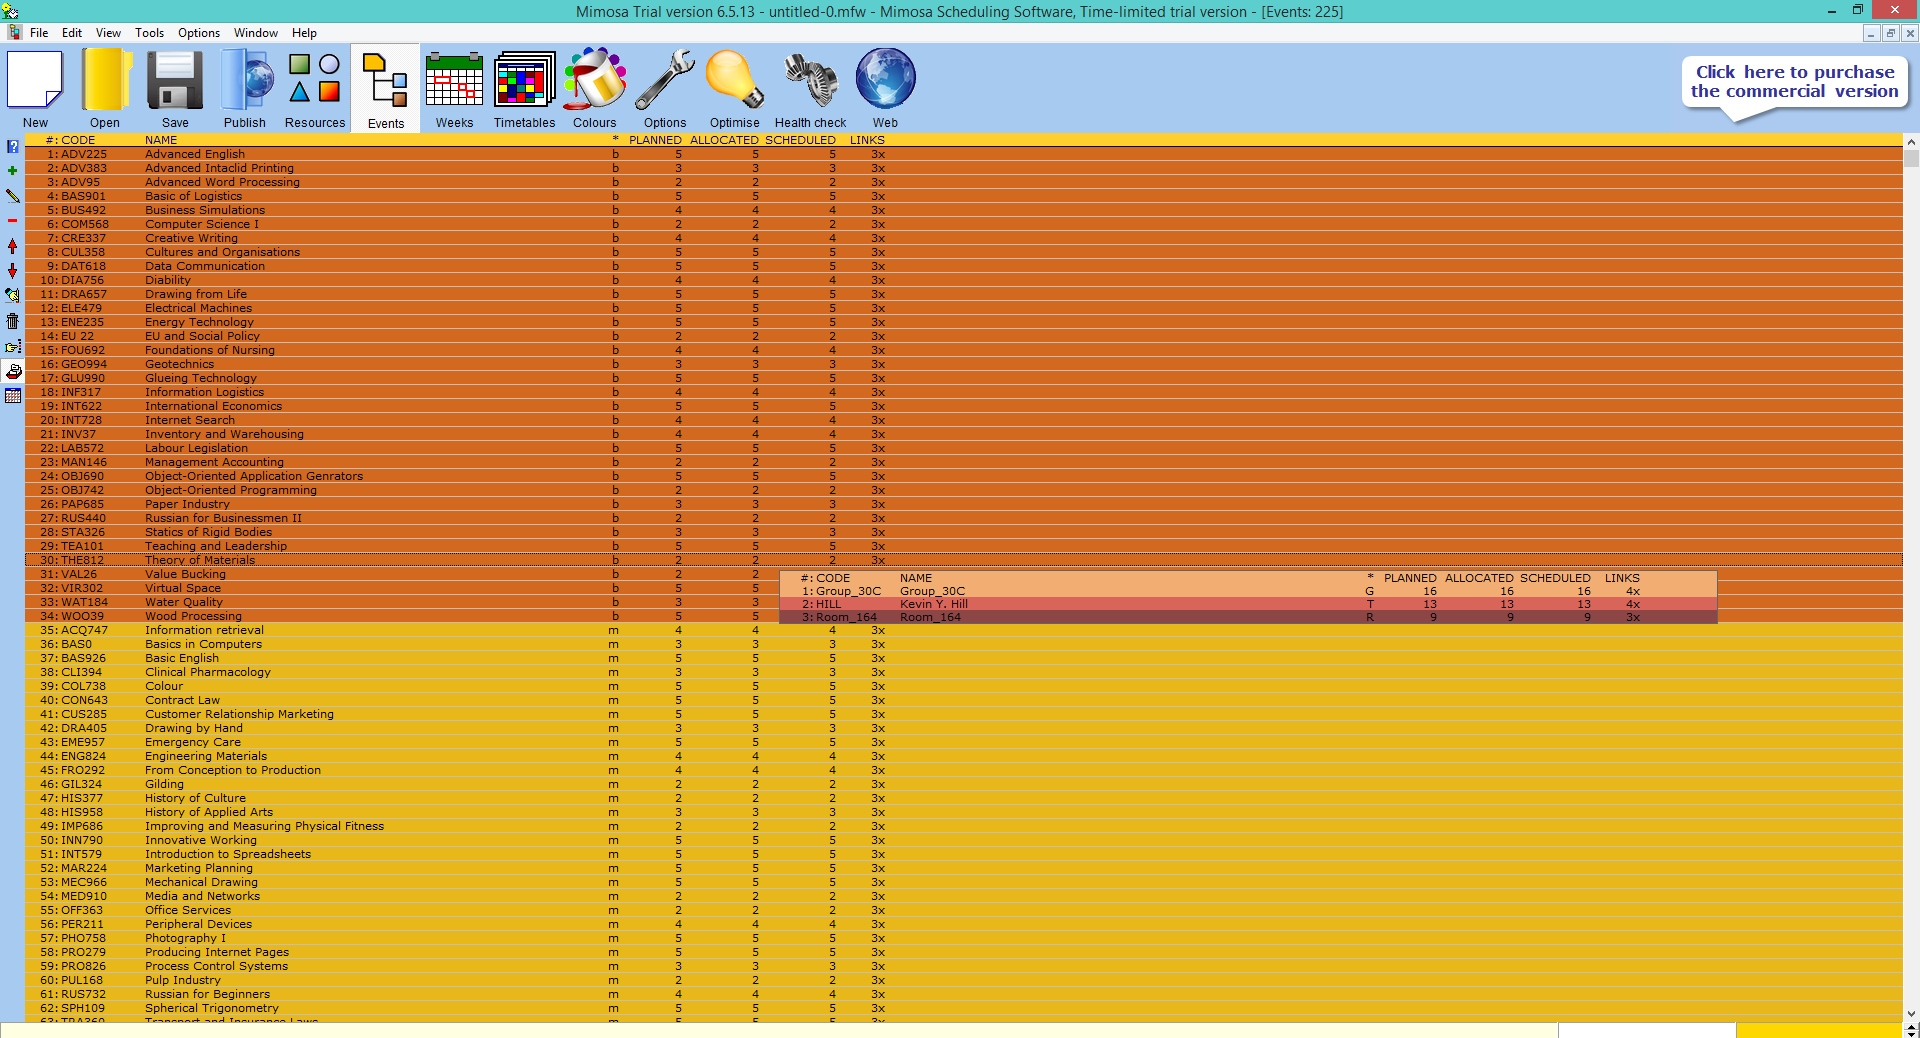
\includegraphics[width=0.5\textwidth]{2}
    }
    }
    \subfigure[Sección de horarios, en la que hemos filtrado el grupo 29C] {
    \label{tabla}
    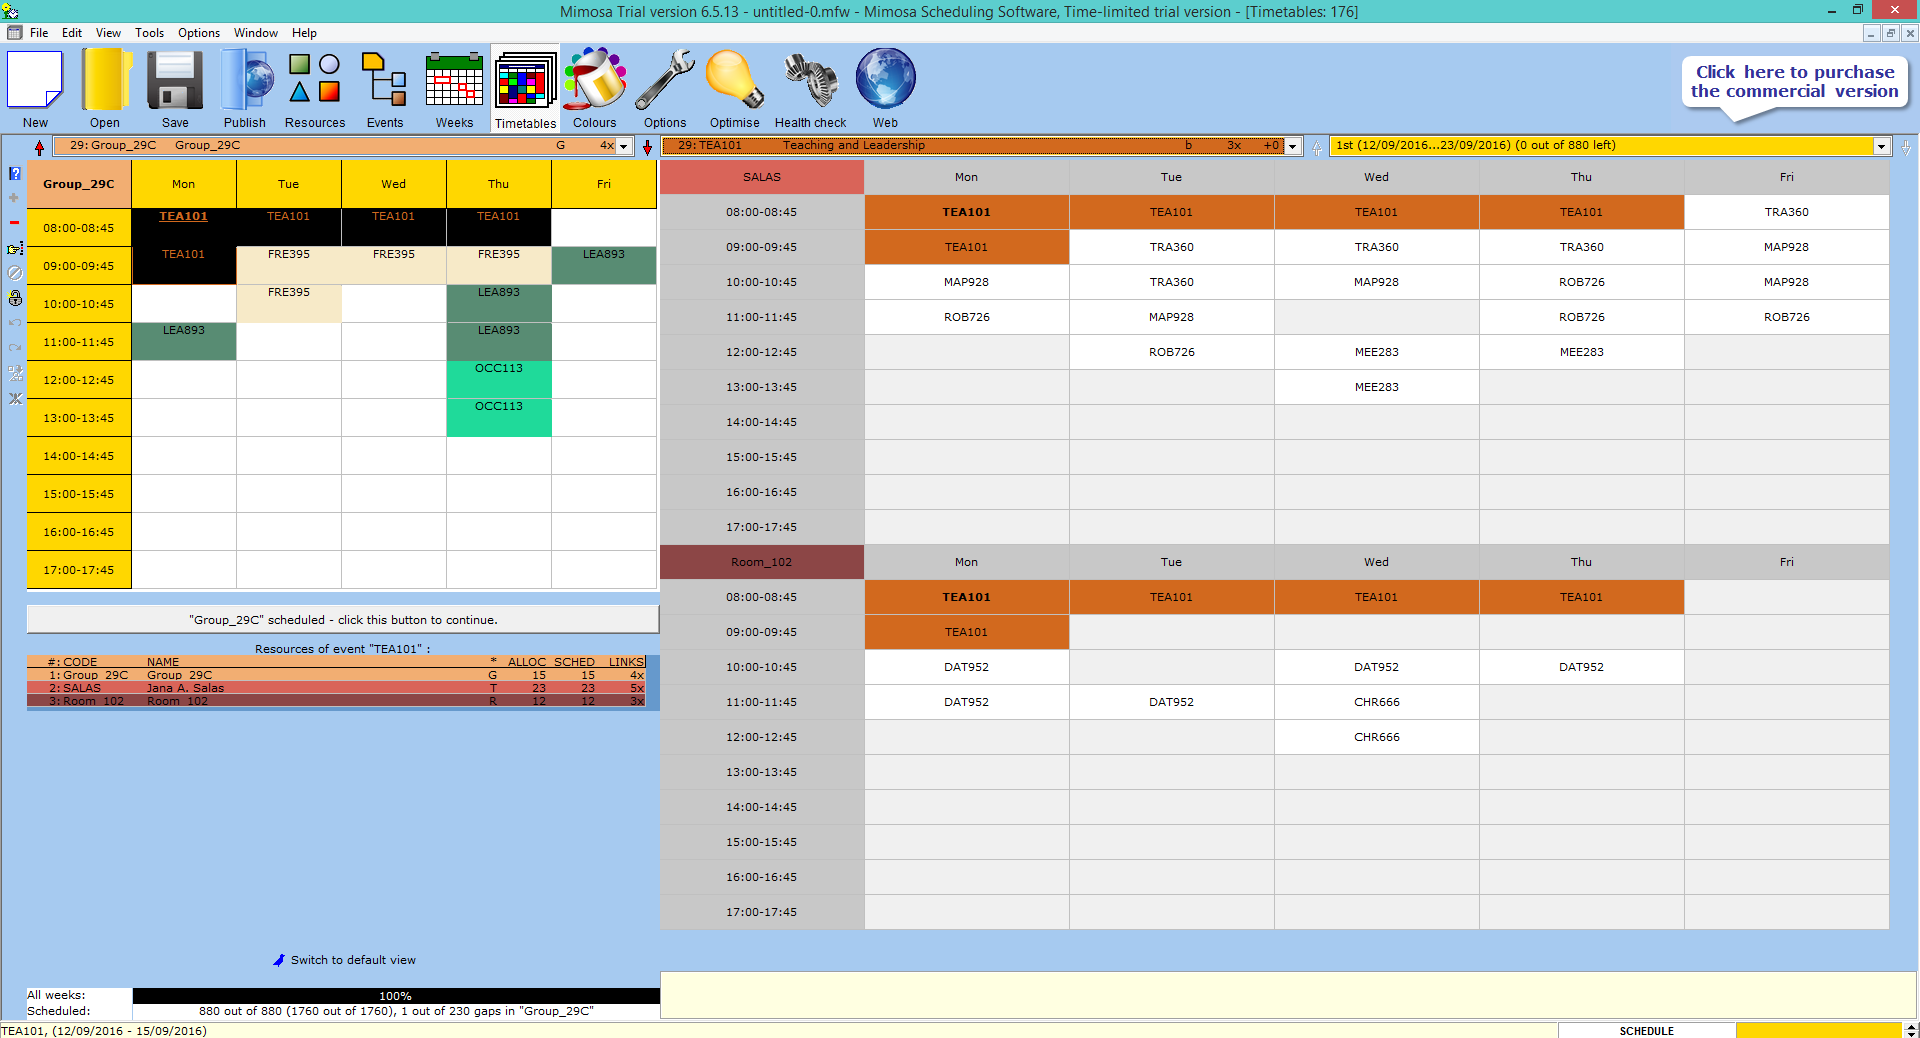
\includegraphics[width=0.5\textwidth]{3}
    }
    \caption{Capturas de pantalla del software \textit{Mimosa}}
    \label{mimosa}
\end{figure}

Por último, \textit{Mimosa} permite exportar el horario generado en distintos formatos tales como \texttt{csv} o web y además de realizar un horario, también permite asignar profesores y alumnos a cada grupo de forma automatizada.

Toda esta información se puede encontrar en su documentación \cite{mimosa}.

\section{Timetabler}

El software llamado \href{http://www.timetabler.com/}{\textit{Timetabler}} es una herramienta para realizar horarios tanto de forma \textbf{no automatizada} (modo interactivo) como de forma \textbf{automatizada}. Incluso permite mezclar ambas, permitiendo que el software realice un horario y el usuario resuelva a mano las posibles incidencias que éste encuentre.

Su modo de funcionamiento se basa en realizar cuatro pasos de forma secuencial:

\begin{enumerate}[1.]
    \item \textbf{Basic data}: en primer lugar, se introduce el profesorado (además del departamento en el que está) y su disponibilidad, los grupos en los que se va a dividir al alumnado, las aulas, las asignaturas a impartir y la estructura del horario (horas en las que se va a dar clase y descansos, días de la semana en los que se va a dar clase, etc). Esta información también puede ser \textbf{importada} desde un fichero.
    \item \textbf{Activities}: a continuación, se describe cada asignatura en términos del número de horas que será impartida. Además, permite ver un resumen de todos los datos introducidos hasta el momento.
    \item \textbf{Schedule}: en este paso, se realiza el horario. Podemos hacerlo de tres formas: manual, semi-automático y automático. 
    \item \textbf{Print}: por último, podemos imprimir el horario en base a una asignatura, un grupo académico, un profesor o un aula. Además, podemos exportar las tablas en distintos formatos y realizar una copia de seguridad.
\end{enumerate}

Una descripción detallada de estos cuatro pasos puede encontrarse en \cite{timetabler}.


% Descripción de sistemas "libres"

\chapter{Otros proyectos libres similares}

A continuación podremos ver algunos de los proyectos que podemos encontrar por \textit{\textbf{Github}} sobre la generación automatizada de horarios.

\section{Plan}

\href{https://github.com/adamcik/plan}{\textit{Plan}} es un software desarrollado como asistente para la creación de horarios de una forma fácil para los estudiantes de \textit{NTNU}, tal y como se puede ver en \cite{plan}.

Esta interfaz web nos pide que creemos un \textit{nick} para poder entrar en la aplicación. Una vez creado, nos pasará a la interfaz que vemos en la \hyperref[plan1]{Figura \ref{plan1}}

\begin{figure}[H]
    \centering
    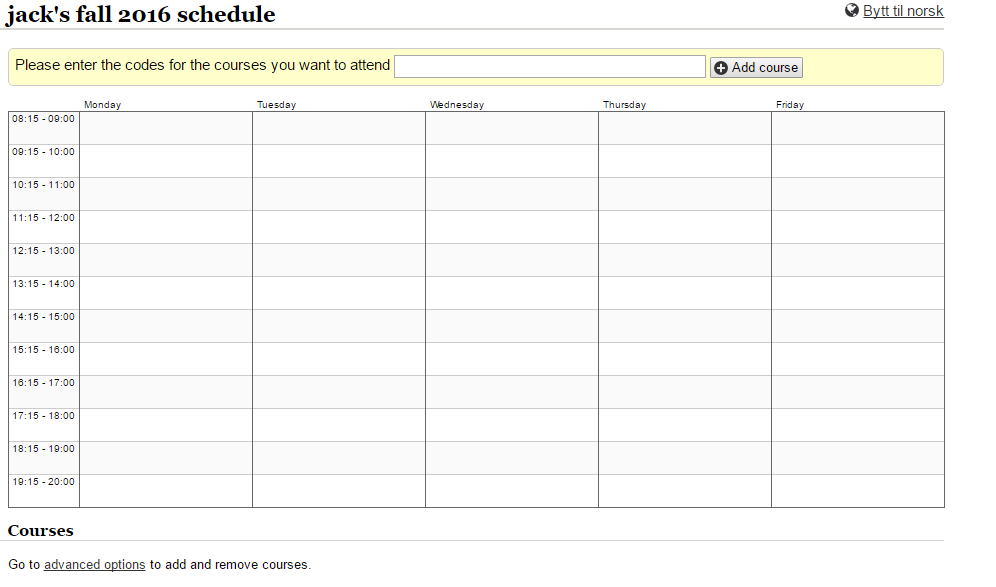
\includegraphics[width=0.7\textwidth]{plan1}
    \label{plan1}
    \caption{Interfaz web para la introducción de las asignaturas}
\end{figure}

En esta interfaz web, tendremos que ir introduciendo los códigos de las asignaturas, generando una tabla de asignaturas en la que el alumno se habrá matriculado, tal y como se puede ver en la \hyperref[plan2]{Figura \ref{plan2}}. En esta tabla, aparecerán los códigos de las asignaturas, su descripción, su fecha de examen y ofrece la posibilidad de dar un alias a la asignatura.

\begin{figure}[H]
    \centering
    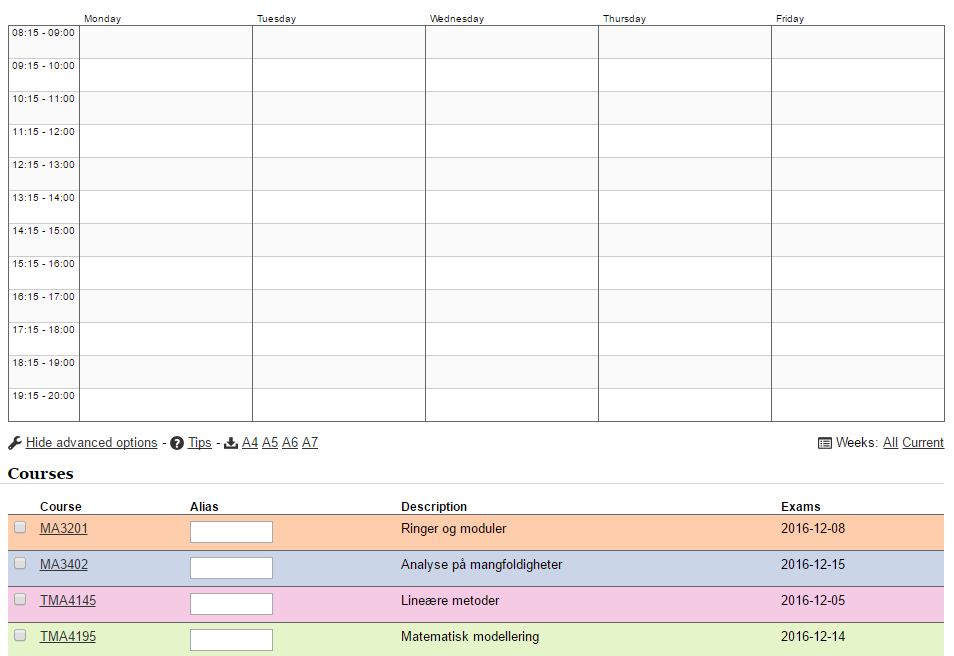
\includegraphics[width=0.7\textwidth]{plan2}
    \label{plan2}
    \caption{Tabla de asignaturas introducidas con sus respectivos códigos}
\end{figure}

Una vez introducidas, el alumno seleccionará los grupos en los que está matriculado y el sistema mostrará automáticamente \textbf{el horario específico para el alumno}. Es decir, dado un alumno con un conjunto de asignaturas $\mathcal{X}$, el sistema mostrará el horario que tiene el alumno en cuestión, como vemos en la \hyperref[plan3]{Figura \ref{plan3}}. A su vez, el sistema ofrece una lista con las clases de cada asignatura y grupo más detallada, como se ve en la \hyperref[plan4]{Figura \ref{plan4}}


\begin{figure}[H]
    \centering
    \mbox {
        
        \subfigure[Horario generado.]{
            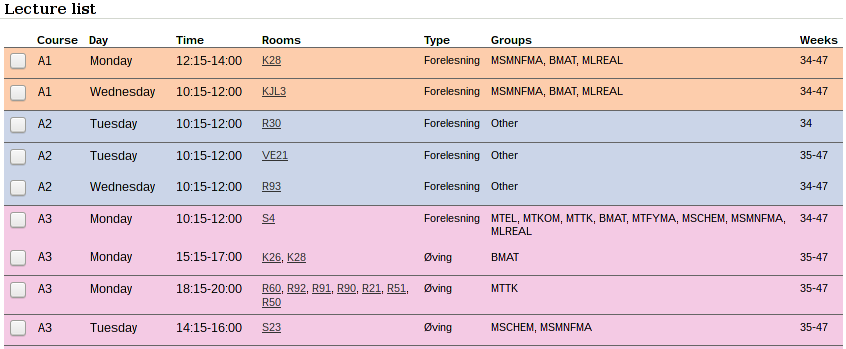
\includegraphics[width=0.5\textwidth]{plan3}
            \label{plan3}
        }
        
        \quad
        
        \subfigure[Lista más detallada de las clases del día.] {
            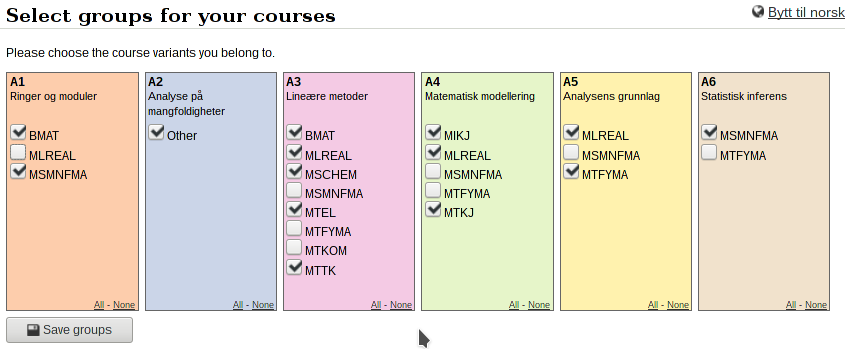
\includegraphics[width=0.5\textwidth]{plan4}
            \label{plan4}
        }
    }
    
    \caption{Horarios y listas que genera el sistema}
    \label{plan3-4}
\end{figure}

Este software ofrece actuálmente varias funciones tales como:

\begin{enumerate}
	\item Una vista personificable del calendario.
	\item Se puede exportar fácilmente a \textit{Google-Calendar}.
	\item Se puede imprimir en formato PDF.
	\item El usuario puede decidir las horas límites.
	\item Permite importar información sobre las asignaturas mediante volcados de una base de datos.
\end{enumerate}

\section{Timetable Generator}

\href{https://github.com/zeus9/timetable_generator}{\textit{Timetable Generator}} es un generador de horarios desarrollado por el usuario \textbf{zeus9} de \textit{Github}. Está desarrollado en C++ y Python 2, haciendo uso de un algoritmo genético para la generación del horario, tal y como se puede ver en \cite{timetableGenerator}.

Este sistema toma como entrada tres ficheros en formato \textbf{\textit{CSV}}, en los que se incluye la siguiente información:

\begin{enumerate}[$\bullet$]
    \item \texttt{initial.csv}: consiste en un fichero que contiene una matriz inicial que conforma el horario. Este horario inicial se utiliza en el algoritmo genético del fichero \textit{labGa.cpp}.
    \item \texttt{periodcount.csv}: supone una relación entre los $ID's$ de los profesores, disponibles en \textit{faculty.csv} y algo más aún por descifrar.
    \item \texttt{labPeriodcount.csv}
\end{enumerate}

Todo esto conforman los datos mínimos de la universidad que necesita el algoritmo para generar el horario. 

Para ejecutar el algoritmo, tiene que ser bajo una distribución Linux, y se realiza ejecutando en un terminal \texttt{./ttgen.sh}. Con esto, aparecerá en pantalla una interfaz muy simple que nos permite configurar los parámetros de ambos algoritmos como se ven en la \hyperref[ttgen1]{Figura \ref{ttgen1}}.

\begin{figure}[H]
    \centering
    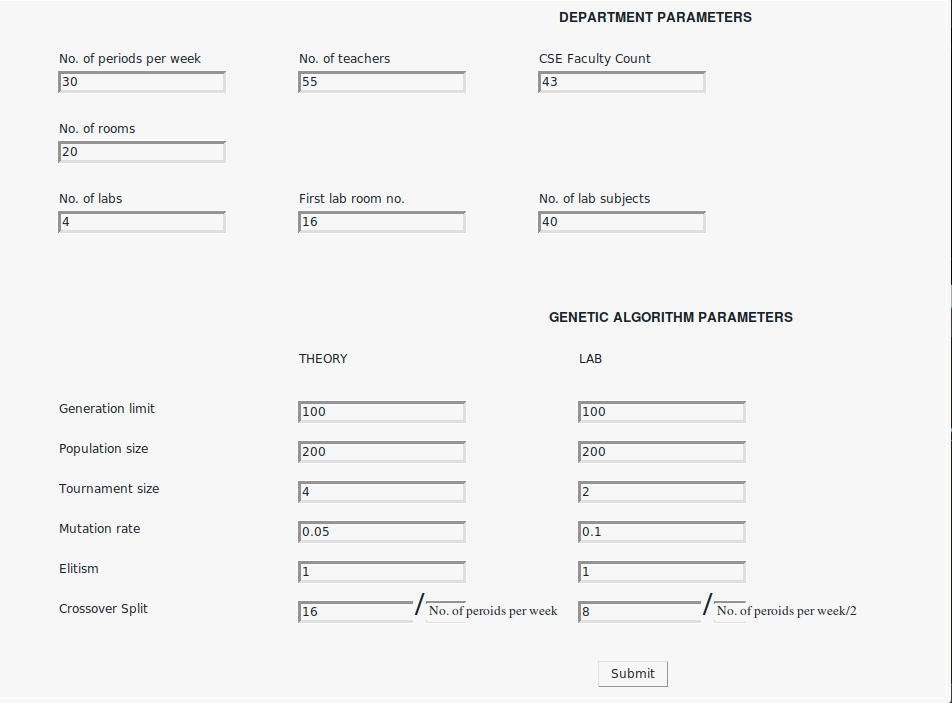
\includegraphics[width=0.7\textwidth]{ttgen1}
    \label{ttgen1}
    \caption{Interfaz para modificar los parámetros del algoritmo genético}
\end{figure}

Tras modificar los parámetros del algoritmo y pulsar el botón \textit{Submit}, estos datos se escriben en el fichero \textit{variables.csv} para el algoritmo genético de \textit{ga.cpp} y en \textit{labVariables.csv} para el algoritmo de \textit{labGa.cpp} y se comienza a ejecutar el $script$ en Python \texttt{labConflictsGen.py} que genera un CSV con las incompatibilidades que pueda haber en las aulas.

A continuación, se ejecuta el algoritmo genético. La variante \texttt{labGa} comienza con un horario inicial de entrada, dando pie al algoritmo genético, a diferencia de \texttt{ga}, que comienza sin un horario de entrada. Al finalizar, ambos muestran por la terminal la solución encontrada, y el coste de esta, siendo a su vez escrito en un fichero.

\section{Unitime}

\href{https://github.com/UniTime/unitime}{\textit{UniTime}} es un sistema que se acerca mucho al sistema deseado, ya que integra un sistema para la generación del horario, asignación de aulas, asignación de exámenes$\ldots$ Permita además modificar la estructura del horario y minimiza los conflictos que existen en el horario.

Este sistema, disponible en \cite{unitime}, está desarrollado en Java, y ofrece una interfaz web simple y con facilidad para moverse entre las opciones.

Este sistema ofrece varios niveles de usuario, partiendo desde un alumno hasta un administrador, con distintos niveles de permisos y acciones, siendo este último el que más acciones disponibles tiene, como son añadir asignaturas, departamentos, aulas y edificios, grupos de estudiantes, etc. 

Además de todo esto, el sistema ofrece una amplia documentación en su página web \href{http://help.unitime.org/}{\textit{http://help.unitime.org/}}, junto con una demo de cada uno de los usuarios posibles que tiene el sistema, para poder probar y ver cada una de las funciones de las que dispone el sistema.

Una característica del sistema es que utiliza internamente un algoritmo de búsqueda local para la satisfacción de restricciones. Este algoritmo consiste en una búsqueda hacia delante iterativa, similar a una búsqueda local, pero con la peculariadad de que el algoritmo puede dar soluciones que no satisfazcan todas las restricciones. Es decir, las restricciones se dividen en restricciones fuertes y restricciones débiles. El algoritmo, satisface todas las restricciones fuertes, pero, las restricciones débiles pueden no ser satisfechas, por lo que el algoritmo explora mejor el espacio de búsqueda obteniendo mejores soluciones, más fáciles de entender para el usuario y con la posiblidad de detener el algoritmo en cualquier momento y devolver una solución al ser iterativo.

% Descripción del sistema

\chapter{Descripción del sistema y requisitos}

\section{Descripción del sistema}

La idea general del sistema es ofrecer una forma automatizada de hacer los horarios de una escuela o facultad en base a restricciones tales como el profesorado y su disponibilidad, las aulas disponibles teniendo en cuenta su capacidad y el equipo del que disponen, el número de alumnos de una asignatura, bloques horarios, etc. 

Con este sistema podrán estudiarse distintas propuestas de horarios para maximizar el uso de las aulas, el rendimiento de todo el equipo de una facultad y facilitar el trabajo que supone la creación de un horario para cada nuevo curso.

\section{Objetivos principales del sistema}

\begin{enumerate}[OBJ-1]
    \item El usuario debe introducir la menor información posible para que le resulte más cómodo y sencillo hacer uso del sistema. Esto sería posible si la mayoría de información necesaria para la generación del horario fuera posible obtenerla de la base de datos de la escuela o de la UGR, para evitar que el usuario tenga que realizar ninguna entrada desde ficheros o similares.
    
    \item Tener la posibilidad de realizar un nuevo horario desde cero a partir de los datos disponibles, y la posibilidad de, a partir de uno ya generado, generar uno nuevo a partir de modificaciones.

    \item Sobre la solución del sistema, existen dos opciones:
    \begin{enumerate}[a)]
        \item Ofrecer una única solución y ofrecer la posibilidad de realizar modificaciones sobre esta de forma interactiva y que el sistema avise de posibles conflictos.
        \item Ofrecer como salida un parapeto de soluciones que haya encontrado el sistema y que el usuario final elija entre las soluciones que más le interesen.
    \end{enumerate}
    % \item Poder conectarse a las bases de datos de la universidad de forma que el usuario introduzca la menor información posible.
    % \item Poder crear un horario válido desde cero usando los datos disponibles.
    % \item Una vez hecha una propuesta de horario, realizar modificaciones sobre la misma de forma que se obtenga un horario válido.
\end{enumerate}

\section{Requisitos del sistema}

\begin{enumerate}[REQ-1]
    \item No pueden solaparse dos asignaturas el mismo día y a la misma hora en el mismo aula.
    \item Cómo máximo hay tres subgrupos de prácticas. Puede haber asignaturas en las que haya dos subgrupos y otras en las que haya sólo uno.
    \item Para cada grupo se debe de decidir de forma manual su franja horaria y el aula de teoría.
    \item No puede haber más de tres grupos de teoría asignados al mismo aula en el mismo turno (mañana o tarde). 
    \item Se debe saber de antemano el número de horas de teoría y prácticas de cada asignatura.
    \item Si el número de horas de teoría o prácticas de una asignatura es impar, se agrupará con otra asignatura que esté en la misma situación. En caso de que no sea posible, ésta hora se añadirá al principio o al final del turno ofreciendo la posibilidad de cambiarla manualmente.
    \item Se debe dar la posibilidad de para una asignatura, dar las horas de teoría en un mismo turno de dos o más horas, o repartir las sesiones de teoría a lo largo de la semana en días distintos.
    \item El horario obtenido para cada grupo no debe de contener huecos, es decir, debe ser lo más compacto posible.
    \item Las distintas especialidades tienen su horario en paralelo para no favorecer ninguna especialidad sobre otra.
    \item Se debe registrar el equipamiento disponible en cada laboratorio y el que cada asignatura necesita para llevar a cabo sus prácticas de forma que el sistema realice la asignación a laboratorios de forma automática.
    \item Se debe poder elegir el número de días y la franja horaria para cada titulación por separado. 
\end{enumerate}


% Primera aproximación greedy

\chapter{Primera aproximación Greedy}
Hemos desarrollado dos algoritmos \textit{Greedy}: uno para asignar las horas de teoría y otro para asignar las horas de prácticas.

\section{Greedy para asignar horas de teoría}
Para inicializar una población para el algoritmo genético, hemos desarrollado un algoritmo \textit{Greedy} aleatorio. El pseudocódigo se ve explicado en el \hyperref[greedyteoria]{Algoritmo \ref*{greedyteoria}} 

\begin{pseudocode}{GreedyTeoria}{ }
    \label{greedyteoria}
    \FOREACH g \in groups \DO
    \BEGIN
        d \GETS 0 \\
        subject\_list \GETS \CALL{shuffle}{\CALL{filter}{subjects, g}}\\
        \WHILE \sum subject\_list.th\_hours \neq 0 \DO
        \BEGIN
            \FOREACH s \in subject\_list \DO
            \BEGIN
                \IF s.th\_hours \neq 0 \DO
                \BEGIN
                    \IF g.turno = ``Morning'' \DO
                    \BEGIN
                        \FOR h \GETS 0 \TO number\_of\_hours / 2 \DO
                        \BEGIN
                            \IF \CALL{libre}{h} \DO
                            \BEGIN
                                tabla[d,h] \GETS (g, s, g.classroom)\\
                                s.th\_hours \GETS s.th\_hours - 1\\
                                d \GETS (d + 1) \bmod number\_of\_days\\
                                \BREAK
                            \END
                        \END
                    \END
                    \ELSE \DO
                    \BEGIN
                        \FOR h \GETS number\_of\_hours / 2 \TO number\_of\_hours \DO
                        \BEGIN
                            \IF \CALL{libre}{h} \DO
                            \BEGIN
                                tabla[d,h] \GETS (g, s, g.classroom)\\
                                s.th\_hours \GETS s.th\_hours - 1\\
                                d \GETS (d + 1) \bmod number\_of\_days\\
                                \BREAK
                            \END
                        \END
                    \END
                \END
            \END
        \END
    \END
\end{pseudocode}

Para realizar el filtrado de asignaturas que pertenecen a cada grupo, filtramos aquellas asignaturas que coincidan tanto en año, como en semestre y especialidad con el grupo en cuestión. Este método pertenece a la clase \texttt{Timetable} y, por tanto, \texttt{tabla}, \texttt{number\_of\_hours} y \texttt{number\_of\_days} son atributos de dicha clase. El atributo \texttt{th\_hours} de la clase \texttt{Subject} corresponde al número de horas teóricas de dicha asignatura.

\subsection{Ejemplo de funcionamiento}
Supongamos que tenemos que hacer un horario para los grupos de segundo curso $A$ y $B$, que están asignados al aula de teoría 0.1 y cuyas asignaturas son:

\begin{enumerate}[$\bullet$]
    \item \textbf{AC} con dos horas de teoría,
    \item \textbf{ALG} con tres horas de teoría y
    \item \textbf{FBD} con una hora de teoría.
\end{enumerate}

Además, también suponemos que el número de días de en los que se quieren cuadrar estas asignaturas es de 3 y 4 horas.

Vamos a hacer los pasos para cuadrar las asignaturas del grupo $A$:

\begin{minipage}{0.5\textwidth}    
\begin{tabular}{| c | c | c |}
\hline
 &  &  \\
 \hline
 &  &  \\
 \hline
 &  &  \\
 \hline
 &  &  \\
 \hline 
\end{tabular}
\end{minipage}
\begin{minipage}{0.5\textwidth}
\begin{tabular}{c | c}
Asignatura & Num horas restantes \\
AC & 2 \\
ALG & 3 \\
FBD & 1
\end{tabular}
\end{minipage}

Seleccionamos la primera asignatura de nuestra lista filtrada y mezclada de asignaturas, \textbf{AC} y colocamos una de sus horas en el primer hueco disponible del horario. 

\begin{minipage}{0.5\textwidth}    
\begin{tabular}{| c | c | c |}
\hline
AC, A, 0.1 &  &  \\
 \hline
 &  &  \\
 \hline
 &  &  \\
 \hline
 &  &  \\
 \hline 
\end{tabular}
\end{minipage}
\begin{minipage}{0.5\textwidth}
\begin{tabular}{c | c}
Asignatura & Num horas restantes \\
AC & 1 \\
ALG & 3 \\
FBD & 1
\end{tabular}
\end{minipage}

Ahora, hacemos lo mismo con \textbf{ALG} y \textbf{FBD}.

\begin{minipage}{0.5\textwidth}    
\begin{tabular}{| c | c | c |}
\hline
AC, A, 0.1 & ALG, A, 0.1  & FBD, A, 0.1 \\
 \hline
 &  &  \\
 \hline
 &  &  \\
 \hline
 &  &  \\
 \hline 
\end{tabular}
\end{minipage}
\begin{minipage}{0.5\textwidth}
\begin{tabular}{c | c}
Asignatura & Num horas restantes \\
AC & 1 \\
ALG & 2 \\
FBD & 0
\end{tabular}
\end{minipage}

Como aún siguen quedando horas por asignar, damos otra vuelta más.

\begin{minipage}{0.5\textwidth}    
\begin{tabular}{| c | c | c |}
\hline
AC, A, 0.1 & ALG, A, 0.1  & FBD, A, 0.1 \\
 \hline
AC, A, 0.1 & ALG, A, 0.1 & ALG, A, 0.1  \\
 \hline
 &  &  \\
 \hline
 &  &  \\
 \hline 
\end{tabular}
\end{minipage}
\begin{minipage}{0.5\textwidth}
\begin{tabular}{c | c}
Asignatura & Num horas restantes \\
AC & 0 \\
ALG & 0 \\
FBD & 0
\end{tabular}
\end{minipage}

Al no quedar más horas por asignar, pasaríamos a repetir estos mismos pasos con el grupo $B$.

\section{Greedy para inicializar horas de prácticas}
En el caso del Greedy para inicializar las horas de prácticas, hemos hecho un algoritmo parecido al de las horas de teoría. Su funcionamiento básico consiste en ir desplazando una ventana, cuyo tamaño será el número de subgrupos de prácticas, e ir asignando dicha ventana cada día de la semana.

\begin{pseudocode}{GreedyPracticas}{ }
    \label{greedypracticas}
    \FOREACH g \in groups \DO
    \BEGIN
        d \GETS 0 \\
        subject\_list \GETS \CALL{shuffle}{\CALL{filter}{subjects, g}}\\
        \WHILE \sum subject\_list.pr\_hours \neq 0 \DO
        \BEGIN
            \FOREACH v \in ventana\_subjects \DO
            \BEGIN
                \IF v.pr\_hours \neq 0 \DO
                \BEGIN
                    \IF g.turno = ``Morning'' \DO
                    \BEGIN
                        \FOR h \GETS 0 \TO number\_of\_hours / 2 \DO
                        \BEGIN
                            \IF \CALL{libre}{h} \DO
                            \BEGIN
                                tabla[d,h] \GETS (g, s)\\
                                s.th\_hours \GETS s.th\_hours - 1\\
                                d \GETS (d + 1) \bmod number\_of\_days\\
                                \BREAK
                            \END
                        \END
                    \END
                    \ELSE \DO
                    \BEGIN
                        \FOR h \GETS number\_of\_hours / 2 \TO number\_of\_hours \DO
                        \BEGIN
                            \IF \CALL{libre}{h} \DO
                            \BEGIN
                                tabla[d,h] \GETS (g, s, g.classroom)\\
                                s.th\_hours \GETS s.th\_hours - 1\\
                                d \GETS (d + 1) \bmod number\_of\_days\\
                                \BREAK
                            \END
                        \END
                    \END
                \END
            \END
        \END
    \END
\end{pseudocode}

\subsection{Ejemplo de funcionamiento}
Supongamos que tenemos que asignar a un grupo con tres subgrupos de prácticas las siguientes asignaturas:

\begin{tabular}{c | c  c  c  c  c}
\textbf{Nombre} & AC & FBD & ALG & IA & FIS \\
\hline
\textbf{Horas de prácticas}  & 2 & 3 & 1 & 2 & 2 \\
\end{tabular}

Al tener tres subgrupos de prácticas, nuestra ventana tendrá tamaño 3. 

\begin{minipage}{0.5\textwidth}    
\begin{tabular}{| c | c | c | c | c |}
\hline
 &  &  &  & \\
 \hline
 &  &  &  & \\
 \hline
 &  &  &  & \\
 \hline
 &  &  &  & \\
 \hline 
\end{tabular}
\end{minipage}
\begin{minipage}{0.5\textwidth}
\begin{tabular}{c | c}
Asignatura & Num horas restantes \\
AC & (2, 2, 2) \\
FBD & (3, 3, 3) \\
ALG & (1, 1, 1) \\
IA & (2, 2, 2) \\
FIS & (2, 2, 2)
\end{tabular}
\end{minipage}

Seleccionamos las tres primeras asignaturas de la lista (AC, FBD, ALG), y las asignamos al primer día de la semana.

\begin{minipage}{0.5\textwidth}    
\begin{tabular}{| c | c | c | c | c |}
\hline
 (AC, A1), &  &  &  & \\
 (FBD, A2), &  &  &  & \\
 (ALG, A3) &  &  &  & \\
 \hline
 (AC, A1), &  &  &  & \\
 (FBD, A2), &  &  &  & \\
 (FBD, A3) &  &  &  & \\
 \hline
 &  &  &  & \\
 \hline
 &  &  &  & \\
 \hline 
\end{tabular}
\end{minipage}
\begin{minipage}{0.5\textwidth}
\begin{tabular}{c | c}
Asignatura & Num horas restantes \\
AC & (0, 2, 2) \\
FBD & (3, 1, 2) \\
ALG & (1, 1, 0) \\
IA & (2, 2, 2) \\
FIS & (2, 2, 2)
\end{tabular}
\end{minipage}

Movemos la ventana en una posición (FBD, ALG, IA) y volvemos a asignar las prácticas para el siguiente día de la semana:

\begin{minipage}{0.5\textwidth}    
\begin{tabular}{| c | c | c | c | c |}
\hline
 (AC, A1), & (FBD, A1), &  &  & \\
 (FBD, A2), & (ALG, A2) &  &  & \\
 (ALG, A3) &  (IA, A3) &  &  & \\
 \hline
 (AC, A1), & (FBD, A1) &  &  & \\
 (FBD, A2), & (FBD, A2) &  &  & \\
 (FBD, A3) & (IA, A3) &  &  & \\
 \hline
 &  &  &  & \\
 \hline
 &  &  &  & \\
 \hline 
\end{tabular}
\end{minipage}
\begin{minipage}{0.5\textwidth}
\begin{tabular}{c | c}
Asignatura & Num horas restantes \\
AC & (0, 2, 2) \\
FBD & (1, 0, 2) \\
ALG & (1, 0, 0) \\
IA & (2, 2, 0) \\
FIS & (2, 2, 2)
\end{tabular}
\end{minipage}

Volvemos a mover la ventana una posición más (ALG, IA, FIS) y repetimos la operación del día anterior. En este caso, el grupo A1 tendrá un hueco en su segunda hora de prácticas, que se rellenará más adelante, si es posible.

\begin{minipage}{0.7\textwidth}    
\begin{tabular}{| c | c | c | c | c |}
\hline
 (AC, A1), & (FBD, A1), & (ALG, A1) &  & \\
 (FBD, A2), & (ALG, A2) & (IA, A2) &  & \\
 (ALG, A3) &  (IA, A3) & (FIS, A3) &  & \\
 \hline
 (AC, A1), & (FBD, A1) & () &  & \\
 (FBD, A2), & (FBD, A2) & (IA, A2) &  & \\
 (FBD, A3) & (IA, A3) & (FIS, A3) &  & \\
 \hline
 &  &  &  & \\
 \hline
 &  &  &  & \\
 \hline 
\end{tabular}
\end{minipage}
\begin{minipage}{0.8\textwidth}
\begin{tabular}{c | c}
Asignatura & Num horas restantes \\
AC & (0, 2, 2) \\
FBD & (1, 0, 2) \\
ALG & (0, 0, 0) \\
IA & (2, 0, 0) \\
FIS & (2, 2, 0)
\end{tabular}
\end{minipage}

Repetimos la operación hasta hacer la semana completa

\begin{minipage}{0.8\textwidth}    
\begin{tabular}{| c | c | c | c | c |}
\hline
 (AC, A1), & (FBD, A1), & (ALG, A1) & (IA, A1) & (FIS, A1) \\
 (FBD, A2), & (ALG, A2) & (IA, A2) & (FIS, A2) & (AC, A2) \\
 (ALG, A3) &  (IA, A3) & (FIS, A3) & (AC, A3) & (FBD, A3) \\
 \hline
 (AC, A1), & (FBD, A1) & () & (IA, A1) & (FIS, A1) \\
 (FBD, A2), & (FBD, A2) & (IA, A2) & (FIS, A2) & (AC, A2) \\
 (FBD, A3) & (IA, A3) & (FIS, A3) & (AC, A3) & (FBD, A3) \\
 \hline
 &  &  &  & \\
 \hline
 &  &  &  & \\
 \hline 
\end{tabular}
\end{minipage}
\begin{minipage}{1\textwidth}
\begin{tabular}{c | c}
Asignatura & Num horas restantes \\
AC & (0, 0, 0) \\
FBD & (1, 0, 0) \\
ALG & (0, 0, 0) \\
IA & (0, 0, 0) \\
FIS & (0, 0, 0)
\end{tabular}
\end{minipage}

Como aún queda una hora por asignar, el algoritmo buscaría un hueco posible donde asignarla.

\begin{minipage}{0.8\textwidth}    
\begin{tabular}{| c | c | c | c | c |}
\hline
 (AC, A1), & (FBD, A1), & (ALG, A1) & (IA, A1) & (FIS, A1) \\
 (FBD, A2), & (ALG, A2) & (IA, A2) & (FIS, A2) & (AC, A2) \\
 (ALG, A3) &  (IA, A3) & (FIS, A3) & (AC, A3) & (FBD, A3) \\
 \hline
 (AC, A1), & (FBD, A1) & (FBD, A1) & (IA, A1) & (FIS, A1) \\
 (FBD, A2), & (FBD, A2) & (IA, A2) & (FIS, A2) & (AC, A2) \\
 (FBD, A3) & (IA, A3) & (FIS, A3) & (AC, A3) & (FBD, A3) \\
 \hline
 &  &  &  & \\
 \hline
 &  &  &  & \\
 \hline 
\end{tabular}
\end{minipage}
\begin{minipage}{1\textwidth}
\begin{tabular}{c | c}
Asignatura & Num horas restantes \\
AC & (0, 0, 0) \\
FBD & (0, 0, 0) \\
ALG & (0, 0, 0) \\
IA & (0, 0, 0) \\
FIS & (0, 0, 0)
\end{tabular}
\end{minipage}

\subsection{Asignación de aulas de prácticas}
Consideramos que la mejor asignación es la que tiene en cuenta el material que necesita cada asignatura para llevar a cabo sus prácticas y el material del que dispone cada aula. Por ejemplo, para la asignatura \textit{Fundamentos de Redes} se necesita usar un aula con una instalación de red especial, por lo que no puede ser asignada en un aula que no disponga de dicha instalación. 

Por tanto, para calcular qué aula es la óptima para cada asignatura, debemos saber qué materiales necesita cada asignatura y qué materiales dispone cada aula. Para saber los materiales de los que dispone cada aula, hemos consultado la página web de la escuela: \url{http://etsiit.ugr.es/pages/instalaciones_servicios/aulas_etsiit2017/!}.

Nuestro algoritmo elige las asignaturas más restrictivas (con una lista de materiales más larga) y les asigna las aulas óptimas. Termina con las asignaturas que \textit{podrían} impartirse en ``cualquier'' aula.

\section{Problemas con esta primera aproximación}
A la hora de implementar esta versión nos hemos encontrado con varios problemas:

\begin{enumerate}[---]
    \item El principal problema de esta forma de asignar los horarios, es que las horas de prácticas se asignaban en la misma franja horaria, es decir, todas las horas de teoría se situaban de 8:30 a 10:30 en el caso del turno de mañana, o de 15:30 a 17:30 en el caso del horario de tarde.

    Esto supone que, las clases de teoría estén muy saturadas, pudiendo darse el caso de que a la misma hora, haya dos grupos de teoría que tengan que dar la clase en el mismo aula, lo que produce una saturación en las aulas de teoría.

    Este problema se agrava mucho más a la hora de asignar las aulas de prácticas, debido al espacio limitado y que todos los grupos de cada turno, comenzaban las prácticas a la misma hora, produciéndose tal saturación, que a la hora de asignar el aula, no acababa en la gran mayoría de los casos, siendo extremadamente difícil asignar aulas a los distintos subgrupos de prácticas de la escuela, y además, realizando una ejecución sólo para el Grado en Ingeniería Informática.

    Un intento de solución que se hizo, que mejoró algo este problema, fue asignar cuándo comenzaban las clases de teoría para cada día lanzando un aleatorio, para elegir si las clases de teoría comenzarían de 8:30 a 10:30, o bien de 10:30 a 12:30, siendo igual para el turno de tarde. 

    En este caso se dio la misma probabilidad a ambas franjas horarias, para no favorecer ninguna y permitir que las clases de prácticas estuvieran más distribuidas y disminuir la saturación de aulas que generaba este algoritmo.

    Esta nueva versión, mejoró algo la situación para los cursos de primero y segundo, teniendo ya algunos problemas para las aulas de tercero, y volviendo a tener los mismos problemas de saturiación para los cursos de cuarto, siendo difícil realizar una asignación de aulas correcta.

    Esto se soluciona haciendo primero una estructura de horarios, en la que hiremos marcando para cada una de las diferentes horas del horario, si corresponde a una hora de teoría de prácticas o de teoría, con el fin de que realizando esta estructura, el algoritmo sea capaz de no sobresaturar las horas de prácticas o teoría. Esto se hace antes de asignar asignaturas tanto de teoría o de prácticas, procurando que si a un grupo a cierta hora le ha asignado una hora de teoría, el siguiente grupo, a esa hora, tendrá una hora de prácticas. Más adelante se podrá encontrar esto con más detalle.

    %En primer lugar, todas las horas de teoría se asignaban en la misma franja horaria, haciendo muy difícil la asigación de aulas de prácticas. Para solucionar esto, antes de empezar a asignar asignaturas con nuestro algoritmo, debemos decidir qué horas son de prácticas y de teoría para cada grupo de forma que, cuando un grupo tenga teoría otro grupo tenga prácticas. Así, la ocupación de las aulas de prácticas se minimiza.

    \item No es posible realizar una asignación óptima de las aulas de prácticas. Esto se debe a que para hacer una asignación óptima de las aulas, es necesario conocer de antemano los materiales de los que dispone cada aula. En el caso de la Escuela Técnica de Ingeniería Informática, es posible obtener la información exacta de cada aula en la página web de la escuela, como hemos mencionado anteriormente.

    El problema está en que cada año este material puede cambiar, al igual que puede cambiar el material que necesita cada asignatura, o cada profesor. Esto hace, que para cada asignatura, cada profesor pueda tener unos requisitos de materiales distintos al resto de profesores para esa asignatura. Por tanto, esto dificulta muchísimo la asignación óptima de aulas de prácticas.

    En nuestra primera aproximación, hicimos una ejecución para crear los horarios sólo del Grado en Ingeniería Informática, donde nosotros asignamos a mano los materiales que necesitaba cada asignatura, muchas por conocimiento propio tras cursar las asignaturas y otras por consultas a compañeros de otras especialidades y de otros años. El resultado tenía cierta aproximación a la asignación de aulas actual, pero no tenía tanta calidad como para presentarlo como resultado final, además de que era para un solo grado. 

    Esto, a la hora de meter más grados, y meter un conocimiento al problema que no era nuestro, comenzó a dar serios problemas para asignar las aulas, ya que había restricciones tan fuertes de materiales, que en algunos casos, ya no era posible asignar las aulas de prácticas, produciendo ciclos y que el programa no acabase en la mayoría de casos, y en los que acababa, el horario resultante, en términos de calidad por horario comprimido y sin huecos en medio de la jornadad, muy malo. 

    Es por esto por lo que decidimos cambiar la forma en la que asignamos las aulas de prácticas, de modo que ya no fuera necesario conocer de forma previa los materiales de las aulas, materiales de cada asignatura, etc. Más adelante, se explicará la siguiente versión del algoritmo para realizar esta tarea, junto con sus ventajas y desventajas.

    %No disponemos de los materiales que necesita cada asignatura para poder hacer sus prácticas. Nuestro tutor nos ha dicho que esta información es bastante difícil de conseguir. Como solución, hemos decidido añadir un requisito: en vez de asignar asignaturas a aulas según material vamos a añadir al Dataset las aulas de prácticas en las que se imparte cada asignatura consultando los actuales horarios.
\end{enumerate}


% Segunda aproximación greey
\chapter{Segunda aproximación Greedy}
% Para resolver los problemas de la primera aproximación realizada, se ha desarrollado un segundo algoritmo greedy. A esta segunda aproximación se le ha añadido un algoritmo previo que sirve para hacer la estructura del horario y cuyo objetivo es minimizar la ocupación de los laboratorios de prácticas.

A raíz de los problemas vistos en la versión anterior, se optó por modificar lo desarrollado hasta ahora y hacer una segunda versión del algoritmo greedy capaz de solventar estos problemas y mejorar la calidad de las soluciones. 

En esta segunda aproximación se realizan varias cosas:

\begin{enumerate}
  \item Simplificación del modelo: se reestructurarán las clases, eliminando elementos innecesarios que aumentan la complejidad del algoritmo y por tanto la complejidad del problema. 
  \item Añadir un paso previo al algoritmo: este paso previo consiste en calcular la estructura básica del horario, preasignando celdas como celdas de teoría o de prácticas, independientemente de la asignatura que se vaya a asignar para facilitar la composición del horario. Más adelante se verá esto con más detalle.
\end{enumerate}

\section{Simplificación del modelo}

Una de las simplificaciones más importantes que se ha hecho del modelo es la eliminación total de los materiales que tiene cada aula y que necesita cada asignatura. Esto aunque pueda parecer muy simple, simplifica enormemente el modelo. 

Esta modificación no se hace así sin más. En vez de haber una lista de materiales posibles que ofrecen las aulas y materiales que necesitan las asignaturas, para después buscar posibles aulas haciendo una intersección, se cambia esto por una lista de aulas en las que se puede impartir una asignatura y se elige una entre las posibles que esté libre. 

Es decir, para aquellas asignaturas que tengan una fuerte restricción de materiales, se les asignará sólo las aulas en las que puedan ser impartidas, y para el resto de asignaturas, se les asignará un aula que esté libre en ese momento entre las distintas aulas de prácticas de las que dispone el centro

Esto sucede en el centro para asignaturas como \textit{Fundamentos Físicos y Tecnológicos}, que necesita aulas con material electrónico, o asignaturas con restricciones más fuertes aún como son \textit{Tecnología y Organización de Computadores} y \textit{Fundamentos de Redes}, que en nuestro centro, no tienen más remedio que ir asignadas al aula 3.10 y 2.7 respectivamente, por las restricciones tan fuertes de materiales que tienen.

Con esto, podemos eliminar los atributos que se usan para almacenar los materiales que necesita cada asignatura, y los materiales de los que dispone cada aula de prácticas, quedando algo como lo que podemos ver en la \hyperref[clases3]{Figura \ref*{clases3}}.

\begin{figure}[H]
  % Graphic for TeX using PGF
% Title: /home/braulio/PycharmProjects/TFG/doc/clases.dia
% Creator: Dia v0.97.3
% CreationDate: Mon Sep  4 20:42:15 2017
% For: braulio
% \usepackage{tikz}
% The following commands are not supported in PSTricks at present
% We define them conditionally, so when they are implemented,
% this pgf file will use them.
\ifx\du\undefined
  \newlength{\du}
\fi
\setlength{\du}{15\unitlength}
\begin{tikzpicture}
\pgftransformxscale{1.000000}
\pgftransformyscale{-1.000000}
\definecolor{dialinecolor}{rgb}{0.000000, 0.000000, 0.000000}
\pgfsetstrokecolor{dialinecolor}
\definecolor{dialinecolor}{rgb}{1.000000, 1.000000, 1.000000}
\pgfsetfillcolor{dialinecolor}
\pgfsetlinewidth{0.100000\du}
\pgfsetdash{}{0pt}
\definecolor{dialinecolor}{rgb}{1.000000, 1.000000, 1.000000}
\pgfsetfillcolor{dialinecolor}
\fill (12.350000\du,4.800000\du)--(12.350000\du,6.200000\du)--(24.015000\du,6.200000\du)--(24.015000\du,4.800000\du)--cycle;
\definecolor{dialinecolor}{rgb}{0.000000, 0.000000, 0.000000}
\pgfsetstrokecolor{dialinecolor}
\draw (12.350000\du,4.800000\du)--(12.350000\du,6.200000\du)--(24.015000\du,6.200000\du)--(24.015000\du,4.800000\du)--cycle;
% setfont left to latex
\definecolor{dialinecolor}{rgb}{0.000000, 0.000000, 0.000000}
\pgfsetstrokecolor{dialinecolor}
\node at (18.182500\du,5.750000\du){Aula};
\definecolor{dialinecolor}{rgb}{1.000000, 1.000000, 1.000000}
\pgfsetfillcolor{dialinecolor}
\fill (12.350000\du,6.200000\du)--(12.350000\du,8.800000\du)--(24.015000\du,8.800000\du)--(24.015000\du,6.200000\du)--cycle;
\definecolor{dialinecolor}{rgb}{0.000000, 0.000000, 0.000000}
\pgfsetstrokecolor{dialinecolor}
\draw (12.350000\du,6.200000\du)--(12.350000\du,8.800000\du)--(24.015000\du,8.800000\du)--(24.015000\du,6.200000\du)--cycle;
% setfont left to latex
\definecolor{dialinecolor}{rgb}{0.000000, 0.000000, 0.000000}
\pgfsetstrokecolor{dialinecolor}
\node[anchor=west] at (12.500000\du,6.900000\du){-tabla\_de\_horas: matrix$<bool>$};
% setfont left to latex
\definecolor{dialinecolor}{rgb}{0.000000, 0.000000, 0.000000}
\pgfsetstrokecolor{dialinecolor}
\node[anchor=west] at (12.500000\du,7.700000\du){+capacidad: uint};
% setfont left to latex
\definecolor{dialinecolor}{rgb}{0.000000, 0.000000, 0.000000}
\pgfsetstrokecolor{dialinecolor}
\node[anchor=west] at (12.500000\du,8.500000\du){+nombre: string};
\pgfsetlinewidth{0.100000\du}
\pgfsetdash{}{0pt}
\definecolor{dialinecolor}{rgb}{1.000000, 1.000000, 1.000000}
\pgfsetfillcolor{dialinecolor}
\fill (14.756600\du,11.342000\du)--(14.756600\du,12.742000\du)--(21.669100\du,12.742000\du)--(21.669100\du,11.342000\du)--cycle;
\definecolor{dialinecolor}{rgb}{0.000000, 0.000000, 0.000000}
\pgfsetstrokecolor{dialinecolor}
\draw (14.756600\du,11.342000\du)--(14.756600\du,12.742000\du)--(21.669100\du,12.742000\du)--(21.669100\du,11.342000\du)--cycle;
% setfont left to latex
\definecolor{dialinecolor}{rgb}{0.000000, 0.000000, 0.000000}
\pgfsetstrokecolor{dialinecolor}
\node at (18.212850\du,12.292000\du){Aula prácticas};
\definecolor{dialinecolor}{rgb}{1.000000, 1.000000, 1.000000}
\pgfsetfillcolor{dialinecolor}
\fill (14.756600\du,12.742000\du)--(14.756600\du,13.142000\du)--(21.669100\du,13.142000\du)--(21.669100\du,12.742000\du)--cycle;
\definecolor{dialinecolor}{rgb}{0.000000, 0.000000, 0.000000}
\pgfsetstrokecolor{dialinecolor}
\draw (14.756600\du,12.742000\du)--(14.756600\du,13.142000\du)--(21.669100\du,13.142000\du)--(21.669100\du,12.742000\du)--cycle;
\pgfsetlinewidth{0.100000\du}
\pgfsetdash{}{0pt}
\pgfsetmiterjoin
\pgfsetbuttcap
{
\definecolor{dialinecolor}{rgb}{0.000000, 0.000000, 0.000000}
\pgfsetfillcolor{dialinecolor}
% was here!!!
\definecolor{dialinecolor}{rgb}{0.000000, 0.000000, 0.000000}
\pgfsetstrokecolor{dialinecolor}
\draw (18.182500\du,8.850250\du)--(18.182500\du,10.470893\du)--(18.212850\du,10.470893\du)--(18.212850\du,11.291536\du);
}
\definecolor{dialinecolor}{rgb}{0.000000, 0.000000, 0.000000}
\pgfsetstrokecolor{dialinecolor}
\draw (18.182500\du,9.762054\du)--(18.182500\du,10.470893\du)--(18.212850\du,10.470893\du)--(18.212850\du,11.291536\du);
\pgfsetmiterjoin
\definecolor{dialinecolor}{rgb}{1.000000, 1.000000, 1.000000}
\pgfsetfillcolor{dialinecolor}
\fill (18.582500\du,9.762054\du)--(18.182500\du,8.962054\du)--(17.782500\du,9.762054\du)--cycle;
\pgfsetlinewidth{0.100000\du}
\pgfsetdash{}{0pt}
\pgfsetmiterjoin
\definecolor{dialinecolor}{rgb}{0.000000, 0.000000, 0.000000}
\pgfsetstrokecolor{dialinecolor}
\draw (18.582500\du,9.762054\du)--(18.182500\du,8.962054\du)--(17.782500\du,9.762054\du)--cycle;
% setfont left to latex
\pgfsetlinewidth{0.100000\du}
\pgfsetdash{}{0pt}
\definecolor{dialinecolor}{rgb}{1.000000, 1.000000, 1.000000}
\pgfsetfillcolor{dialinecolor}
\fill (26.600000\du,4.750000\du)--(26.600000\du,6.150000\du)--(39.805000\du,6.150000\du)--(39.805000\du,4.750000\du)--cycle;
\definecolor{dialinecolor}{rgb}{0.000000, 0.000000, 0.000000}
\pgfsetstrokecolor{dialinecolor}
\draw (26.600000\du,4.750000\du)--(26.600000\du,6.150000\du)--(39.805000\du,6.150000\du)--(39.805000\du,4.750000\du)--cycle;
% setfont left to latex
\definecolor{dialinecolor}{rgb}{0.000000, 0.000000, 0.000000}
\pgfsetstrokecolor{dialinecolor}
\node at (33.202500\du,5.700000\du){Grupo};
\definecolor{dialinecolor}{rgb}{1.000000, 1.000000, 1.000000}
\pgfsetfillcolor{dialinecolor}
\fill (26.600000\du,6.150000\du)--(26.600000\du,9.550000\du)--(39.805000\du,9.550000\du)--(39.805000\du,6.150000\du)--cycle;
\definecolor{dialinecolor}{rgb}{0.000000, 0.000000, 0.000000}
\pgfsetstrokecolor{dialinecolor}
\draw (26.600000\du,6.150000\du)--(26.600000\du,9.550000\du)--(39.805000\du,9.550000\du)--(39.805000\du,6.150000\du)--cycle;
% setfont left to latex
\definecolor{dialinecolor}{rgb}{0.000000, 0.000000, 0.000000}
\pgfsetstrokecolor{dialinecolor}
\node[anchor=west] at (26.750000\du,6.850000\du){+nombre: string};
% setfont left to latex
\definecolor{dialinecolor}{rgb}{0.000000, 0.000000, 0.000000}
\pgfsetstrokecolor{dialinecolor}
\node[anchor=west] at (26.750000\du,7.650000\du){+franja\_horaria: pair$<uint, uint>$};
% setfont left to latex
\definecolor{dialinecolor}{rgb}{0.000000, 0.000000, 0.000000}
\pgfsetstrokecolor{dialinecolor}
\node[anchor=west] at (26.750000\du,8.450000\du){+num\_subg\_pract: uint};
% setfont left to latex
\definecolor{dialinecolor}{rgb}{0.000000, 0.000000, 0.000000}
\pgfsetstrokecolor{dialinecolor}
\node[anchor=west] at (26.750000\du,9.250000\du){+curso: unsigned int};
\pgfsetlinewidth{0.100000\du}
\pgfsetdash{}{0pt}
\definecolor{dialinecolor}{rgb}{1.000000, 1.000000, 1.000000}
\pgfsetfillcolor{dialinecolor}
\fill (18.350000\du,16.250000\du)--(18.350000\du,17.650000\du)--(30.015000\du,17.650000\du)--(30.015000\du,16.250000\du)--cycle;
\definecolor{dialinecolor}{rgb}{0.000000, 0.000000, 0.000000}
\pgfsetstrokecolor{dialinecolor}
\draw (18.350000\du,16.250000\du)--(18.350000\du,17.650000\du)--(30.015000\du,17.650000\du)--(30.015000\du,16.250000\du)--cycle;
% setfont left to latex
\definecolor{dialinecolor}{rgb}{0.000000, 0.000000, 0.000000}
\pgfsetstrokecolor{dialinecolor}
\node at (24.182500\du,17.200000\du){Asignatura};
\definecolor{dialinecolor}{rgb}{1.000000, 1.000000, 1.000000}
\pgfsetfillcolor{dialinecolor}
\fill (18.350000\du,17.650000\du)--(18.350000\du,21.050000\du)--(30.015000\du,21.050000\du)--(30.015000\du,17.650000\du)--cycle;
\definecolor{dialinecolor}{rgb}{0.000000, 0.000000, 0.000000}
\pgfsetstrokecolor{dialinecolor}
\draw (18.350000\du,17.650000\du)--(18.350000\du,21.050000\du)--(30.015000\du,21.050000\du)--(30.015000\du,17.650000\du)--cycle;
% setfont left to latex
\definecolor{dialinecolor}{rgb}{0.000000, 0.000000, 0.000000}
\pgfsetstrokecolor{dialinecolor}
\node[anchor=west] at (18.500000\du,18.350000\du){+num\_horas\_teoria: uint};
% setfont left to latex
\definecolor{dialinecolor}{rgb}{0.000000, 0.000000, 0.000000}
\pgfsetstrokecolor{dialinecolor}
\node[anchor=west] at (18.500000\du,19.150000\du){+num\_horas\_pract: uint};
% setfont left to latex
\definecolor{dialinecolor}{rgb}{0.000000, 0.000000, 0.000000}
\pgfsetstrokecolor{dialinecolor}
\node[anchor=west] at (18.500000\du,19.950000\du){+aulas\_posibles: list$<string>$};
% setfont left to latex
\definecolor{dialinecolor}{rgb}{0.000000, 0.000000, 0.000000}
\pgfsetstrokecolor{dialinecolor}
\node[anchor=west] at (18.500000\du,20.750000\du){+curso: uint};
\pgfsetlinewidth{0.100000\du}
\pgfsetdash{}{0pt}
\definecolor{dialinecolor}{rgb}{1.000000, 1.000000, 1.000000}
\pgfsetfillcolor{dialinecolor}
\fill (28.547000\du,11.775000\du)--(28.547000\du,13.175000\du)--(37.902000\du,13.175000\du)--(37.902000\du,11.775000\du)--cycle;
\definecolor{dialinecolor}{rgb}{0.000000, 0.000000, 0.000000}
\pgfsetstrokecolor{dialinecolor}
\draw (28.547000\du,11.775000\du)--(28.547000\du,13.175000\du)--(37.902000\du,13.175000\du)--(37.902000\du,11.775000\du)--cycle;
% setfont left to latex
\definecolor{dialinecolor}{rgb}{0.000000, 0.000000, 0.000000}
\pgfsetstrokecolor{dialinecolor}
\node at (33.224500\du,12.725000\du){SubGrupoPracticas};
\definecolor{dialinecolor}{rgb}{1.000000, 1.000000, 1.000000}
\pgfsetfillcolor{dialinecolor}
\fill (28.547000\du,13.175000\du)--(28.547000\du,14.975000\du)--(37.902000\du,14.975000\du)--(37.902000\du,13.175000\du)--cycle;
\definecolor{dialinecolor}{rgb}{0.000000, 0.000000, 0.000000}
\pgfsetstrokecolor{dialinecolor}
\draw (28.547000\du,13.175000\du)--(28.547000\du,14.975000\du)--(37.902000\du,14.975000\du)--(37.902000\du,13.175000\du)--cycle;
% setfont left to latex
\definecolor{dialinecolor}{rgb}{0.000000, 0.000000, 0.000000}
\pgfsetstrokecolor{dialinecolor}
\node[anchor=west] at (28.697000\du,13.875000\du){-subgrupo\_de: Grupo};
% setfont left to latex
\definecolor{dialinecolor}{rgb}{0.000000, 0.000000, 0.000000}
\pgfsetstrokecolor{dialinecolor}
\node[anchor=west] at (28.697000\du,14.675000\du){-horas\_y\_aula\_asignadas};
\pgfsetlinewidth{0.100000\du}
\pgfsetdash{}{0pt}
\pgfsetmiterjoin
\pgfsetbuttcap
{
\definecolor{dialinecolor}{rgb}{0.000000, 0.000000, 0.000000}
\pgfsetfillcolor{dialinecolor}
% was here!!!
\definecolor{dialinecolor}{rgb}{0.000000, 0.000000, 0.000000}
\pgfsetstrokecolor{dialinecolor}
\draw (33.202500\du,9.600299\du)--(33.202500\du,11.062448\du)--(33.224500\du,11.062448\du)--(33.224500\du,11.724597\du);
}
\definecolor{dialinecolor}{rgb}{0.000000, 0.000000, 0.000000}
\pgfsetstrokecolor{dialinecolor}
\draw (33.202500\du,10.512102\du)--(33.202500\du,11.062448\du)--(33.224500\du,11.062448\du)--(33.224500\du,11.724597\du);
\pgfsetmiterjoin
\definecolor{dialinecolor}{rgb}{1.000000, 1.000000, 1.000000}
\pgfsetfillcolor{dialinecolor}
\fill (33.602500\du,10.512102\du)--(33.202500\du,9.712102\du)--(32.802500\du,10.512102\du)--cycle;
\pgfsetlinewidth{0.100000\du}
\pgfsetdash{}{0pt}
\pgfsetmiterjoin
\definecolor{dialinecolor}{rgb}{0.000000, 0.000000, 0.000000}
\pgfsetstrokecolor{dialinecolor}
\draw (33.602500\du,10.512102\du)--(33.202500\du,9.712102\du)--(32.802500\du,10.512102\du)--cycle;
% setfont left to latex
\end{tikzpicture}

  \caption{Nueva estructura de clases y atributos.}
  \label{clases3}
\end{figure}

Esto tiene una serie de consecuencias y una de ellas es que el espacio de búsqueda para realizar una asignación de aulas crece, por lo que el problema, en la teoría, se dificulta. En la práctica sucede que al tener menos restricciones, podemos simplemente asignar una asignatura a cualquier aula que esté libre, siempre y cuando no se infrinja la condición de que las asignaturas con más restricciones de aulas como las que hemos visto anteriormente tengan asignadas las aulas esperadas.

Otra consecuencia derivada de esta decisión es que el espacio en memoria que necesita la máquina para ejecutar el algoritmo se reduce enormemente al no tener que almacenar listas de materiales para todas y cada una de las asignaturas, al igual que con las distintas aulas. Esto supone que máquinas con muchas menos prestaciones que las máquinas en las que se ha desarrollado el proyecto, puedan ejecutar el algoritmo sin problemas al necesitar menos memoria. También se mejora el tiempo de ejecución, ya que no se producen tantos accesos a memoria, tanto para consultar como para escribir a las distintas listas de materiales, etc.

\section{Preasignación de horas}
Ante la aparición de estos problemas en la primera versión del algoritmo, decidimos volver a analizar el problema y reestructurar los algoritmos, obteniendo una nueva versión del algoritmo greedy. Para llevar a cabo esta tarea, tuvimos varias reuniones con Dº Jesús García Miranda, para hablar sobre los problemas que tenía la primera versión, y discutir nuevas soluciones a este problema. 

Una de las soluciones principales que nos dio, fue la de generar una estructura de datos auxiliar en la que se calculará una estructura preliminar del horario. En ella se asignarán qué casillas de las que hay en el horario se clasifican como clases de teoría y cuáles como clases de prácticas. Esto se hace con el fin de evitar una saturación en las aulas del centro, haciendo que si un grupo $x$ tiene una clase de teoría en el momento $(d, h)$, un grupo $x'$ tendrá en ese momento clase de prácticas, optimizando de esta forma el espacio.

Esta preasignación en el horario se hace sólo teniendo en cuenta el número de horas de teoría y prácticas totales que tiene un grupo concreto para un curso, en vez de ir mirando asignatura por asignatura. De esta forma se obtiene una visión mucho más global del problema y se empieza a construir una buena solución desde el momento inicial del algoritmo, lo que hace que sea más fácil obtener buenas soluciones, a pesar de que esto suponga también limitar el espacio de búsqueda del problema. El objetivo de esta fase es simplemente minimizar la ocupación de los laboratorios de prácticas y teoría, evitando una saturación de las aulas del centro y optimizar los espacios de este.

A su vez, esto nos permite simplificar mucho el algoritmo, porque aunque hay que añadir una fase más al algoritmo, las fases siguientes sólo tienen que completar ``el puzzle con pistas'' que nos ha dejado esta fase, simplificando tanto la estructura de los algoritmos, tiempos de ejecución, consumo de memoria, etc.

Por sencillez, se ha decidido que este algoritmo sólo calcula una franja, en vez de las dos para que el algoritmo sea más simple. Esta franja se decide mediante un parámetro en el que se establece la franja horaria (mañana o tarde). Es por esto, por lo que deben filtrarse los grupos y trabajar con aquellos que pertenezcan al turno que se está calculando. Una vez filtrados estos grupos, el algoritmo irá calculando la estructura para cada uno de los cursos que corresponden.

El algoritmo antes de comenzar el bucle principal, realiza una serie de cálculos. Para empezar, calcula el número total de horas de teoría y prácticas que tiene para cada curso. Además de esto, hay que calcular el número de horas totales libres de laboratorio que hay, para comprobar si en algún momento en el horario habrá grupos que tengan en el mismo instante de tiempo prácticas a la vez. Por ejemplo, si los laboratorios están abiertos cinco días a la semana y cuatro horas al día tendríamos un total de 20 horas. Como cada turno de prácticas tiene dos horas, nos quedarían un total de diez turnos de prácticas por asignar. Si, por ejemplo, tuviésemos que asignar doce turnos de prácticas, tendríamos que elegir de forma aleatoria dos turnos de prácticas que se repetirían. Debe ser de forma aleatoria para que los turnos ``repetidos'' no coincidan en los distintos cursos y se saturen los laboratorios un día en concreto.

Después, el algoritmo empieza a iterar sobre cada grupo de ese curso y va asignando horas de prácticas y teoría en los huecos ``libres''. Para saber qué huecos están libres se usa una matriz auxiliar que registra qué horas son de prácticas en cada curso.

\subsection{Pseudocódigo del algoritmo}
El siguiente pseudocódigo refleja de forma más clara el funcionamiento de este algoritmo:

\begin{pseudocode}{GreedyEstructura}{turno}
\label{greedyestructura}
filtro\_grupos \GETS \CALL{FiltrarGrupos}{turno}\\
principio \GETS \CALL{ComienzoFranja}{turno}\\
final \GETS \CALL{FinalFranja}{turno}\\
\FOREACH curso \in cursos \DO
\BEGIN
    filtro\_cursos \GETS \CALL{FiltrarGruposCurso}{curso, filtro\_grupos}\\
    h\_lab \GETS \CALL{CalcularHorasPracticasCurso}{curso}\\
    h\_week \GETS dias\_semana \cdot n\_turnos\\

    \IF h\_lab > h\_week \THEN
	    	dias\_rep \GETS \CALL{CalcularTurnosRepetidos}{ }
    \ELSE 
      dias\_rep \GETS \emptyset\\

   	tabla\_lab \GETS \CALL{Matriz}{dias\_semana, n\_turnos, value=False}\\

   	\FOREACH g \in filtro\_cursos \DO
   	\BEGIN
   		teoria \GETS \CALL{CalcularHorasTeoria}{g}\\
   		lab \GETS \CALL{CalcularHorasLab}{g}\\

   		\FOR hora \GETS 0 \TO final; i+=2 \DO
   		\BEGIN
   		   \FOR dia \in SEMANA \DO
           \BEGIN
                \IF \NOT tabla\_lab[hora, dia] \AND lab \ge 2 \THEN
                \BEGIN
                    \CALL{AsignarEstructura}{hora, dia, L}\\
                    tabla\_lab[hora, dia] = True\\
                    tabla\_lab[hora + 1, dia] = True\\
                    lab \GETS lab - 2\\
                \END
                \ELSEIF tabla\_lab[hora, dia] \AND lab \ge 2 \AND (dia, hora) \in dias\_rep \THEN
                \BEGIN
                    \CALL{delete}{dias\_rep(dia, hora)}\\
                    \CALL{AsignarEstructura}{hora, dia, L}\\
                    lab \GETS lab - 2\\
                \END
                \ELSEIF tabla\_lab[hora, dia] \AND teoria \ge 2 \THEN
                \BEGIN
                    \CALL{AsignarEstructura}{hora, dia, T}\\
                    teoria \GETS teoria - 2\\
                \END
                \ELSEIF teoria \ge 2 \THEN
                \BEGIN
                    \CALL{AsignarEstructura}{hora, dia, T}\\
                    teoria \GETS teoria - 2\\
                \END
                \ELSEIF lab \ge 2 \THEN
                \BEGIN
                    \CALL{AsignarEstructura}{hora, dia, L}\\
                    lab \GETS lab - 2\\
                \END
                \ELSEIF teoria = 1 \THEN
                \BEGIN
                  \CALL{AsignarEstructura}{hora, dia, T}\\
                  teoria \GETS teoria - 1\\
                \END
                \ELSEIF lab = 1 \THEN
                \BEGIN
                  \CALL{AsignarEstructura}{hora, dia, L}\\
                  lab \GETS lab - 1\\
                \END
                \ELSE \CALL{break}{}
           \END
   		\END
   	\END
\END
\end{pseudocode}

El algoritmo comienza filtrando los grupos según el turno que se esté calculando, además de caclcular el punto de partida y final para el bucle interno en función del turno, para no tener que estar constantemente calculándolo. Una vez pasado esto, pasamos al bucle principal.

Dentro del bucle principal, lo que hace el algoritmo es calcular el número de horas de prácticas que tiene el grupo y el número de horas totales que hay en una semana. En caso de que las horas de prácticas del grupo sean mayores que las que hay disponibles para una asignatura, se escogerá un día aleatorio de la semana en el que se va a repetir un turno.

\section{Asignación de horas de teoría}
Esta segunda versión del algoritmo de asignación de horas de teoría utiliza como base la estructura hecha por el algoritmo de preasignación. Así, sólo tiene permitido asignar horas en los huecos que estén marcados como \texttt{T} en la matriz de estructura. Usando esto como base y un diccionario con las horas por asignar de cada asignatura, el algoritmo distingue varios casos diferentes:

\begin{enumerate}[---]
  \item Si la hora actual no se corresponde a una de teoría en la matriz de estructura, el algoritmo no hace nada.
  \item Si la hora actual sí es de teoría y además la asignatura a asignar tiene más de dos horas pendientes por asignar, se crea un bloque de dos horas con dicha asignatura.
  \item Si la hora actual sí es de teoría pero la asignatura a asignar sólo tiene una hora más por asignar, el algoritmo trata de buscar otra con la que hacer un bloque de dos. En el caso de no existir, se asignaría esa hora únicamente.
\end{enumerate}

Cuando a una asignatura no le quedan más horas por asignar, se elimina automáticamente de la lista de asignaturas por asignar. El algoritmo pasa al siguiente grupo cuando dicha lista se queda vacía.

\subsection{Comparación con la primera versión}
En comparación con la primera versión, hay bastantes cosas que hemos mejorado:

\begin{enumerate}[$\bullet$]
  \item En la versión anterior, si no se conseguía hacer un bloque de dos con dos horas sueltas, el algoritmo o bien ciclaba o bien dejaba huecos en el horario, dando lugar a una estructura no deseada.
  \item En consecuencia, el algoritmo es más rápido que el anterior desarrollado.
  \item Usando el algoritmo de preasignación, hemos conseguido que el código sea mucho más sencillo y legible.
  \item También, el algoritmo ha perdido esa alta diversidad que tenía la versión original puesto que en la nueva versión se ha acotado mucho la estructura del algoritmo y el espacio de búsqueda.
\end{enumerate}

En conclusión, aunque el algoritmo haya perdido su diversidad original, hemos ganado tanto en eficiencia como en calidad.

\subsection{Pseudocódigo del algoritmo}
El siguiente pseudocódigo refleja de forma más clara el funcionamiento del algoritmo.

\begin{pseudocode}{GreedyTeoria}{ }
\label{greedyteoria}
\FOREACH g \in grupos
\BEGIN
  subject\_list \GETS \CALL{ObtenerListaAsignaturas}{g}\\
  \CALL{Barajar}{subject\_list}\\
  horas \GETS \CALL{DiccionarioHoras}{subject\_list}\\
  s \GETS 0\\

  \IF g.turno = M \THEN
  \BEGIN
    empezar \GETS 0 \\
    acabar \GETS \frac{horas\_dia}{2}\\
  \END
  \ELSE 
  \BEGIN
    empezar \GETS \frac{horas\_dia}{2}\\
    acabar \GETS horas\_dia\\
  \END\\

  \FOR h \GETS empezar \TO acabar; h+=2\\
  \BEGIN
    \FOR d \GETS 0 \TO W_d
    \BEGIN
      \IF subject\_list = \emptyset \THEN
      \BREAK\\

      \ELSEIF \NOT (\CALL{EsTeoria}{g, h, d} \AND \\ \;\;\; \CALL{EsTeoria}{g,h+1,d}) \THEN
      \BEGIN
        remove \GETS \FALSE\\
        asignado \GETS \FALSE\\
      \END\\

      \ELSEIF \CALL{EsTeoria}{g, h, d} \AND \\ \;\;\; horas[subject\_list[s]] \geq 2 \THEN
      \BEGIN
        eliminar \GETS \CALL{AsignarCeldaT}{g,h,d,2}\\
        asignado \GETS \TRUE\\
      \END\\

      \ELSEIF \CALL{EsTeoria}{g, h, d} \AND \\ \;\;\; horas[subject\_list[s]] = 1 \THEN
      \BEGIN
        eliminar \GETS \CALL{AsignarCeldaT}{g,h,d,1}\\
        asignado \GETS \TRUE\\
      \END\\
      \ELSEIF \CALL{EsTeoria}{g, h+1, d} \AND \\ \;\;\; horas[subject\_list[s]] = 1 \THEN
      \BEGIN
        eliminar \GETS \CALL{AsignarCeldaT}{g,h+1,d,1}\\
        asignado \GETS \TRUE\\
      \END\\

      \IF eliminar \THEN \CALL{EliminarAsignaturasCero}{ }\\
      \ELSE s = s+1 \pmod{subject\_list.size()}\\
    \END
  \END 
\END
\end{pseudocode}

\section{Asignación de horas de prácticas}

\subsection{Análisis de la versión anterior}

Esta nueva versión del algoritmo voraz para asignar las horas de prácticas y aulas a los distintos grupos, sigue la misma filosofía de la utilización de la ``\textit{ventana}'' para asignar los grupos. 

En la versión anterior, lo que se hacía era, partiendo de una permutación inicial de las distintas asignaturas que tenía el grupo en un cuatrimiestre dado, se generaba una nueva permutación en la que los elementos de esta eran grupos de tres asignaturas o tantas como subgrupos de prácticas haya, que se correspondían con la asignación de las asignaturas, para cada día. A continuación, podemos ver un ejemplo de lo que realizaba esta ventana:
\begin{table}[H]
\begin{center}
\begin{tabular}{|c|c|c|c|c|}
\hline
FFT & CA & ALEM & FS & FP\\
\hline
\end{tabular}
\caption{Permutación inicial.}
\end{center}
\end{table}
Al haber en primero tres subgrupos de prácticas, tenemos lo siguiente:
\begin{table}[H]
\begin{center}
\begin{tabular}{|c|c|c|c|}
\hline
(FFT, CA, ALEM) & (CA, ALEM, FS) & (ALEM, FS, FP) & $\cdots$ \\
\hline
\end{tabular}
\caption{Permutaciones generadas por la ventana.}
\end{center}
\end{table}

Con esto, podríamos ver cómo el primer día de prácticas correspondería a Fundamentos Físicos y Tecnológicos para el grupo 1, Cálculo para el grupo 2 y Álgebra Lineal y Estructuras Matemáticas para el grupo 3.

Esto hace que asignar las horas de prácticas a los distintos días de la semana sea muy fácil, ya que, a partir de una permutación inicial, vamos moviendo una ventana que toma $n$ asignaturas, y se va desplazando una posición a la derecha para cada día de la semana. 

El problema que tiene el realizar la asignación de esta forma, como se hacía en la primera versión, es que si todas las asignaturas del plan de estudio tuvieran la misma cantidad de horas de prácticas y teoría, esta asignación funcionaría sin problemas ninguno. Esto sería el caso ideal, pero la realidad no es así, sino que en un mismo año del plan de estudios, para un semestre dado, podemos encontrarnos asignaturas con una, dos o incluso tres horas de prácticas en un mismo grupo, por lo que este algoritmo, en esta versión tan simple, no funciona. 

Además de esto, el consumo de memoria de esta versión del algoritmo es muy elevado, ya que a partir de la permutación inicial, generar una nueva lista con las ternas de asignaturas, supone repetir varias veces el mismo elemento, lo que supone un mal gasto de memoria innecesario, que podría hacer que máquinas con menor potencia de cálculo y/o recursos, se vean afectadas en su rendimiento.

\subsection{Formulación de la siguiente versión}

Teniendo estos problemas en mente de la versión anterior, procedimos a realizar una nueva versión del algoritmo de prácticas. Esta nueva versión parte desde un punto más ventajoso que la versión original, gracias a la preasignación de celdas, el algoritmo solo tiene que ir mirando qué celdas de la estructura del horario son para prácticas y cuáles no, y asignar las asignaturas donde corresponda.

La elección de qué asignaturas van a cada día, se realizará con la misma idea que la versión anterior, utilizando la ventana deslizante. Pero en este caso, la idea se ha refinado mucho más que la versión anterior. 

La diferencia más básica es que ya no se genera una lista con ternas de asignaturas, sino lo que se mantiene es una lista de índices, que marcan qué asignatura va para cada grupo, y se va sumando uno módulo número de asignaturas del grupo, para ese cuatrimestre. Esto reduce la memoria y simplifica mucho el código.



%% Bibliografía y referencias
\bibliography{bibliografia.bib} %archivo citas.bib que contiene las entradas 
\bibliographystyle{siam} % hay varias formas de citar
\end{document}
